\begin{figure}[H]
    \centering
    \begin{subfigure}{0.48\columnwidth}
        \centering
        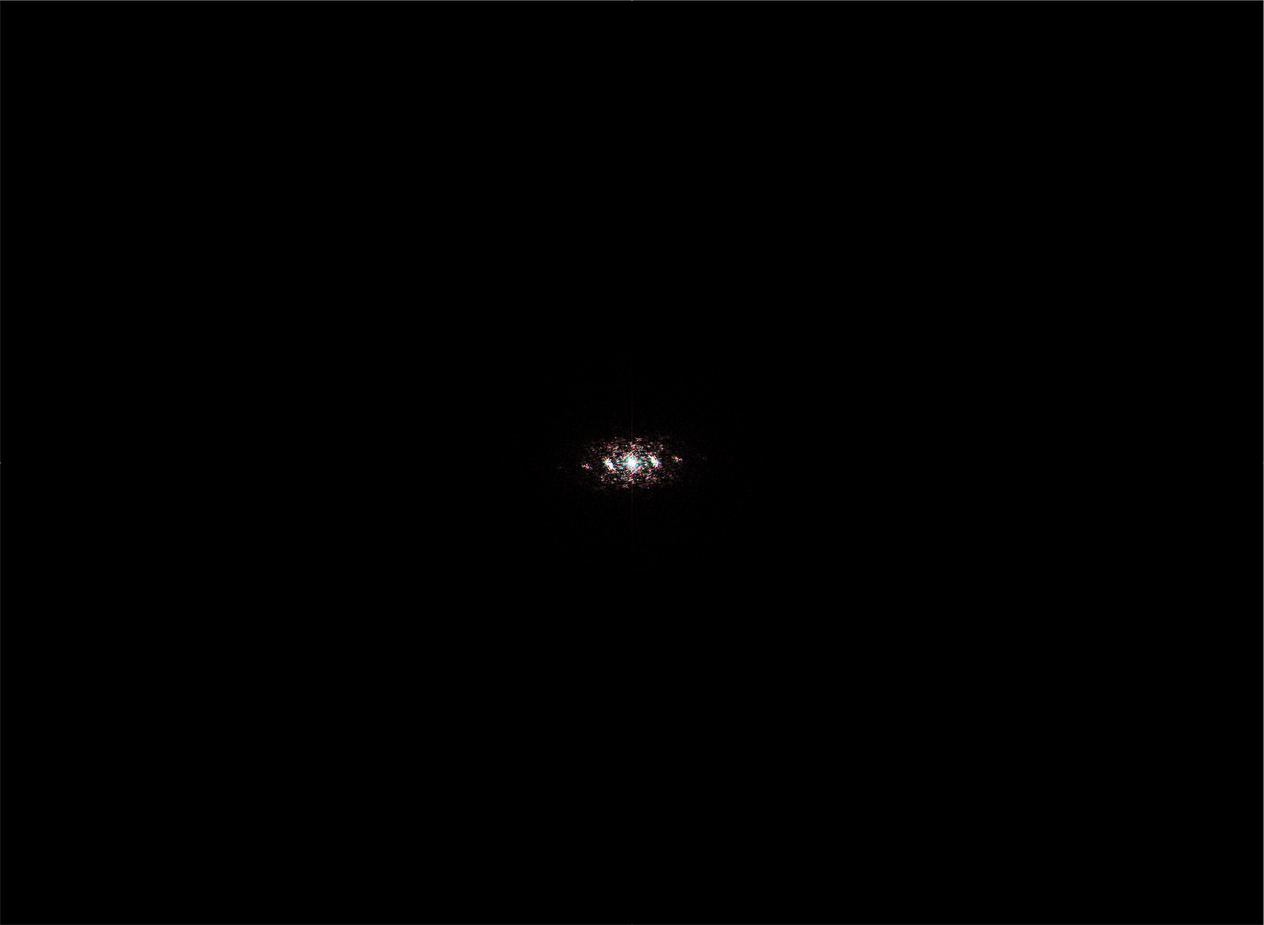
\includegraphics[width=0.9\columnwidth]{figures/expantion fourie transform.png}
        \caption{inverse discrete fourie transform calculated from the interference pattern at of the helix }
        \label{fig:expansion inverse fourie transform measured}
    \end{subfigure}\hfill
    \begin{subfigure}{0.48\columnwidth}
        \centering
        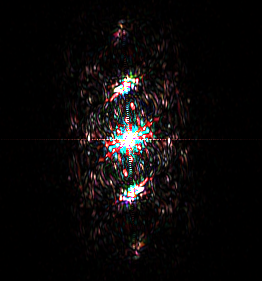
\includegraphics[width=\columnwidth]{figures/expantion fourie transform magnified.png} % second figure itself
        \caption{magnification of \ref{fig:expansion inverse fourie transform measured}}
        \label{fig:expansion fourie transform magnified}
    \end{subfigure}

    \label{fig:expansion theory measurements}
\end{figure}
